\chapter{Approach}
\label{ch:approach}

% \instructions{Page budget for Approach: 20-30 pages
% %
% \begin{itemize}
%     \item This chapter describes your main contributions (i.e., what you did) and the decisions that went into them (i.e., why did you did it the way you did it).
%     \item Alternative headings may be used depending on the kind of contribution(s) you make.
% \end{itemize}
% }

\section{Overview}
% \instructions{
% \begin{itemize}
%     \item This section should explain the high-level design
%     \item Include possibly an architecture figure that shows how the different parts fit together and what processing/technology/tools/datasets have been used for the different components.
% \end{itemize}
% %
% Name these themes based on the different components or sub-problems you are solving in your thesis.
% }

The Automatic Generation of Presentations for Research Papers (AGPRP) generates presentations in \LaTeX{} Beamer format from academic research papers. It comprises three main components: a report parser, a presentation generator, and a presentation compiler. The report parser is responsible for extracting the relevant information from the report, the presentation generator is responsible for generating the presentation, and the presentation compiler is responsible for compiling the presentation into a \LaTeX{} Beamer file. The system is designed to be modular, so each component can be replaced with a different implementation. This allows for easy extension of the system, as well as for easy testing of different approaches.

A two-step approach is suggested for generating the slides: first, the high-level topics are identified and used to generate slide titles, then bullet points are generated for each slide. An optional third step is to generate visual content for the slides, such as tables and illustrations.

\begin{figure}
    \centering
    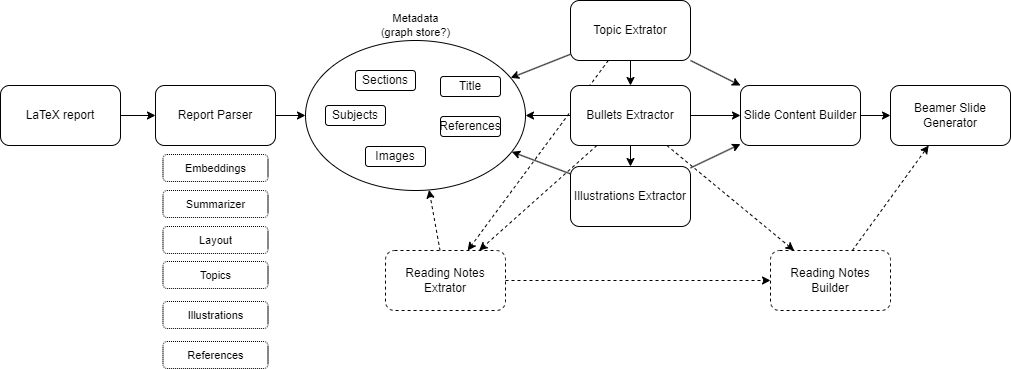
\includegraphics[width=1\linewidth]{images/High-Level Architecture Diagram.png}
    \caption{High-level architecture.}
    \label{fig:high-level-architecture}
\end{figure}

%
\subsection{NOTES (Section to be deleted)}
\begin{itemize}
    \item Could it be beneficial to use a knowledge graph to represent the information in the report? This could be used to generate the presentation and provide a visual representation of the information in the report.
    \item Summarizing vs extracting information from the report. How do we decide the best approach?
    \item Should we test various models, e.g., HuggingFace transformers vs ChatGPT?
    \item Testing how well already existing models (e.g., ChatGPT, MS Copilot) perform when asked to generate a presentation from a research paper.
    \item How do we identify the main file when using LaTeX as the source file? Where do we start parsing? 
    \item Extract the outline from PDF/PPT titles, add additional metadata (e.g., bullets, tables, illustrations), and generate slides from an outline. (Few-shot prompting LLM?) (Manually procure a high-quality dataset)
\end{itemize}

\section{Dataset}

A major contribution of this thesis is the creation of a dataset of research papers and their corresponding presentations. The dataset will be used to train and evaluate the system. The dataset will be created by collecting research papers and their corresponding presentations from various sources. The dataset will be in \LaTeX{} format for the reports and in PDF/PPT format for the presentations. Ideally, the reports and the presentations should be in LaTeX format, but corresponding presentations in the wanted format have proven challenging to find in practice. 

Some datasets are already available, as shown in chapter \ref{ch:related}, but they are not in the format we need. However, they can be used as a starting point for creating the dataset by using the presentations and mining the corresponding research papers in the required format. The arXiv archive is a good source for research papers, and the dataset can be created by mining the arXiv archive for research papers available in \LaTeX{} format. It's important to adhere to the copyrights for the scraped data if we want to publish the dataset. We also need to follow the data scraping guidelines put forth by arXiv.

\subsection{Data Collection}
Since a prerequisite for the dataset is that the research papers are in \LaTeX{} format and the presentations are in \LaTeX{} Beamer format, we need to find a source for research papers and presentations in the required formats. The arXiv archive is a good source for research papers, and part of the dataset can be created by mining the arXiv archive for research papers available in \LaTeX{} format. However, obtaining the corresponding presentations in the required format has proven challenging. Most authors don't seem to publish the corresponding presentations for their research papers. After visisting the personal websites for a selection of authors, the ratio of presentations to research papers are less than 1:10. Based on this we decided that the best approach would be to start with the presentations and mine the corresponding research papers in the required format. Also, the few presentations that are available are often in PDF or PPT format. This means that we need to convert the presentations to the required format. 

We base our data collection on the conference papers from the dataset provided by \citet{Fu:2022:AAAI}. A web scraper was created using the Python Scrapy framework\footnote{\url{https://scrapy.org/}}, that starts by searching for links to available presentations in the event archives. Then, for each presentation found, we use the Python arxiv library\footnote{\url{https://pypi.org/project/arxiv/}} to search for the corresponding research paper in the arXiv archive. If we get an exact match between the titles from both sources, we download the presentation in PDF format, and the matched paper in both PDF and source format. Note that the source files may not be guaranteed to be in \LaTeX{} format, so we need to check that before using the source files in later processing.

In addition some papers and presentations will be manually added to the dataset. This will be done to ensure that the dataset is of high quality and to ensure that the dataset is diverse and representative of the research papers and presentations that the system will be used on.

\subsection{Extracting data from PDF documents}
Since we start out with presentaions and reports in 

\subsection{Data Preprocessing}
If we need to work with PDF formats, we must convert them to \LaTeX{} format before training our model on the dataset. 

\subsection{Data Augmentation}
Enriching the dataset with details such as internal and external references, tables, and illustrations may be useful. This can help generate the presentation, as it can be used to determine which additional items to include together with the text.

\section{Tools}

\subsection{\LaTeX{}}
Parsing \LaTeX{} documents may be done using the TexSoup Python library\footnote{\url{https://texsoup.alvinwan.com/}}.

\subsection{PDF}
Several tools may be able to convert PDF files into text or \LaTeX{} format: 

\begin{itemize}
    \item https://github.com/kermitt2/grobid - ''A machine learning software for extracting information from scholarly documents''
    \item \textbf{PDFMiner}\footnote{\url{https://pypi.org/project/pdfminer/}} - PDFMiner is a tool for extracting information from PDF documents. Unlike other PDF-related tools, it focuses entirely on getting and analyzing text data. PDFMiner lets one obtain the exact text location on a page and other information, such as fonts or lines. It includes a PDF converter that can transform PDF files into other text formats (such as HTML). It has an extensible PDF parser that can be used for purposes other than text analysis.
    \item \textbf{pdftolatex}\footnote{\url{https://github.com/vinaykanigicherla/pdftolatex}} - ''Python tool for generating \LaTeX{} code from PDF files.''
    \item \textbf{pdf2latex-converter}\footnote{\url{https://github.com/mcpeixoto/pdf2latex-converter}} - ''Originally based on \textbf{pdftolatex}.'' (Work in progress).
    \item \textbf{pdf2latex}\footnote{\url{https://github.com/emsquid/pdf2latex}} - ''pdf2latex is a CLI tool to convert a PDF back to LaTeX.''
    \item \textbf{pdf2latex}\footnote{\url{https://github.com/safnuk/pdf2latex}} - ''Train a neural network to produce latex source code which generates a given pdf file.''
    \item \textbf{PDF2LaTeX}\footnote{\url{https://github.com/senyalin/PDF2LaTeX}} - PDF2LaTeX is a tool for converting PDF files into \LaTeX{} format. It is a command-line tool that can convert PDF files into \LaTeX{} format. It is written in Python and uses the PyPDF2 library to parse PDF files. It can be used to convert PDF files into \LaTeX{} format.
    \item \textbf{pypdf}\footnote{\url{https://pypi.org/project/pypdf/}} - pypdf is a Python library for working with PDF files. It can be used to extract text from PDF files and convert PDF files into other formats (such as HTML).
    \item \textbf{pdfly}\footnote{\url{https://github.com/py-pdf/pdfly}} - ''CLI tool to extract (meta)data from PDF and manipulate PDF files.''
\end{itemize}

\section{Baseline}
In order to set a baseline for the system, we use the dataset and trained models provided by \citep{Fu:2022:AAAI}. The dataset contains 5873 pairs of research papers and presentations, and the authors have published their trained models and complete dataset online. As shown in Table \ref{table:dataset} the reports are in PDF format, and the presentation slides are in JPEG format. 

\section{Method}

\subsection{Report Parser (RP)}
The \emph{Report Parser (RP)} is responsible for extracting the relevant information from the report. The report parser comprises two main components: the \emph{Report Content Extractor (RCE)} and the \emph{Report Content Summarizer (RCS)}. The \emph{Report Content Extractor} is responsible for extracting the relevant information from the report, while the \emph{Report Content Summarizer} summarizes the extracted information.

\subsection{Presentation Content Generator}
The \emph{Presentation Content Generator (PCG)} is responsible for 
Presentations can be generated in various layouts, content, and style variations. 

\subsection{Presentation Slides Generator}
There are several options for generating visual layout and content for the presentation slides. 

To keep things simple, we propose three simple slide layouts: A title slide, a bullet point slide, and a visual slide. The title slide will contain the title, the bullet point slide will contain a list of bullet points, and the visual slide will represent the information in the report.

% \instructions{
% \begin{itemize}
%     \item For larger/more complex projects, the separate themes may be chapters on their own (e.g., components in a system; sub-problems of a major evaluation study; etc.).
%     \item Include screenshots, examples, tables, algorithms (with pseudo code), plots for some preliminary observations leading to some aspect of your approach decisions, etc. so that it's not just text.
%     \item Always discuss the alternatives considered and the rationale for the choosing the solutions you adopted.
% \end{itemize}
% }
% %
